Read over the concepts in this chapter and answer the following questions:
\begin{enumerate}
  \item What values can a Boolean expression have?
  \item What are the values of the following expressions?
  
  \begin{table}[h]
    \centering
    \begin{tabular}{|c|l|l|}
      \hline
      \textbf{Question} & \textbf{Expression} & \textbf{Given} \\
      \hline
      (a) & \texttt{1 > 5} & \\
      \hline
      (b) & \texttt{1 < 5} & \\
      \hline
      (c) & \texttt{a > b} & \texttt{a} is 1 and \texttt{b} is 2 \\
      \hline
      (d) & \texttt{(a > b) or (b > a)} & \texttt{a} is 1 and \texttt{b} is 2 \\
      \hline
      (e) & \texttt{(a > b) and (b > a)} & \texttt{a} is 2 and \texttt{b} is 2 \\
      \hline
      (f) & \texttt{a or b or c} & \texttt{a} is False, \texttt{b} is False, and \texttt{c} is True\\
      \hline
      (g) & \texttt{(a or b) and (c or d)} & \texttt{a} is False, \texttt{b} is True, \texttt{c} is True, and \texttt{d} is False \\
      \hline
      (h) & \texttt{(a or b) and (c or d)} & \texttt{a} is False, \texttt{b} is True, \texttt{c} is False, and \texttt{d} is False \\
      \hline
      (i) & \texttt{(a and b) or (c and d)} & \texttt{a} is False, \texttt{b} is True, \texttt{c} is True, and \texttt{d} is True \\
      \hline
      (j) & \texttt{a xor b} & \texttt{a} is True and \texttt{b} is True\\
      \hline
      (k) & \texttt{(a or b) and (not (a and b))} & \texttt{a} is True and \texttt{b} is True\\
      \hline
      (l) & \texttt{not True} & \\
      \hline
      (m) & \texttt{a and (not b)} & \texttt{a} is True and \texttt{b} is False\\
      \hline
    \end{tabular}    
  \end{table}
  
  \csection{
    The following table shows the C syntax for these boolean expressions.\newline\newline
    \begin{tabular}{|c|l|}
      \hline
      \textbf{Question} & \textbf{Expression} \\
      \hline
      (a) & \texttt{1 > 5} \\
      \hline
      (b) & \texttt{1 < 5} \\
      \hline
      (c) & \texttt{a > b} \\
      \hline
      (d) & \texttt{(a > b) || (b > a)} \\
      \hline
      (e) & \texttt{(a > b) \&\& (b > a)} \\
      \hline
      (f) & \texttt{a || b || c} \\
      \hline
      (g) & \texttt{(a || b) \&\& (c || d)} \\
      \hline
      (h) & \texttt{(a || b) \&\& (c || d)} \\
      \hline
      (i) & \texttt{(a \&\& b) || (c \&\& d)} \\
      \hline
      (j) & \texttt{a \^{} b} \\
      \hline
      (k) & \texttt{(a || b) \&\& (!(a \&\& b))} \\
      \hline
      (l) & \texttt{!false} \\
      \hline
      (m) & \texttt{a \&\& (!b)}\\
      \hline
    \end{tabular}
  }
  
  \item What are the two kinds of branching statements?
  \item What are the differences between these statements?
  \item When would you use each of these kinds of branching statements?
  \item What are the two different kinds of looping statements?
  \item What are the differences between these statements?
  \item When would you use each of these kinds of looping statements?
  \item How do Boolean expressions relate to branching and looping statements?
  \item What are the four jumping statements?
  \item What are the differences between these statements?
  \item Why do you need compound statements? Where would these be used?
  \item In structured programming, what are the three different kinds of blocks?
  \item How many entry/exits are there from these blocks?
  \item What are the principles of structured programming?
  \item How does this influence the way you design programs?
  \item Open a new SwinGame project and examine the startup code. How does this program keep the window open until the user closes it?
\end{enumerate}

\clearpage

Use what you have learnt to read and understand the following code samples.
\begin{enumerate}
  \item Read the C code in \lref{clst:rect-move}, or the Pascal code in \lref{plst:rect-move}, and then answer the following questions:
  \begin{enumerate}
    \item What are \texttt{X\_SPEED}, \texttt{width}, \texttt{height}, \texttt{x}, and \texttt{y}? How are they similar/different? What purpose does each of these play? What values are they assigned?
    \item What does the loop in this code do?
    \item Briefly explain what this code does, and suggest a name for the \texttt{????} procedure.
    \item Provide an example of how you could call this procedure.
  \end{enumerate}
  
  \begin{figure}[h]
    \csection{\ccode{clst:rect-move}{What does this C code do?}{topics/control-flow/exercises/rect_move.c}}
  \end{figure}
  \begin{figure}[h]
    \passection{\pascode{plst:rect-move}{What does this Pascal code do?}{topics/control-flow/exercises/RectMove.pas}}
  \end{figure}
  
  \item Read the C code in \lref{clst:color-pick}, or the Pascal code in \lref{plst:color-pick}, and then answer the following questions:
  \begin{enumerate}
    \item What will be drawn to the screen when the user is not holding down any key?
    \item When the user is holding down the G key what will be drawn?
    \item When the user is holding down the R and B keys what will be drawn?
    \item What condition causes the loop to end? How can a user end this loop?
    \item Draw a flow chart to illustrate the possible paths through this code.
  \end{enumerate}
  \begin{figure}[h]
    \csection{\ccode{clst:color-pick}{What does this C code do?}{topics/control-flow/exercises/color_pick.c}}
  \end{figure}
  \begin{figure}[h]
    \passection{\pascode{plst:color-pick}{What does this Pascal code do?}{topics/control-flow/exercises/ColorPick.pas}}
  \end{figure}
  \clearpage
  
  \item Read the C code in \lref{clst:bar_pattern}, or the Pascal code in \lref{plst:bar_pattern}, and then answer the following questions:
  \begin{enumerate}
    \item What do the local variables and parameter keep track of?
    \item How many times will the loop execute?
    \item What is the purpose of the if statement within the loop?
    \item What will be drawn to the screen when this procedure is called?
  \end{enumerate}
  \begin{figure}[h]
    \csection{\ccode{clst:bar_pattern}{What does this C code do?}{topics/control-flow/exercises/draw_bar_pattern.c}}
  \end{figure}
  \begin{figure}[h]
    \passection{\pascode{plst:bar_pattern}{What does this Pascal code do?}{topics/control-flow/exercises/DrawBarPattern.pas}}
  \end{figure}
  \clearpage
  
  \item Read the C code in \lref{clst:color-pick1}, or the Pascal code in \lref{plst:color-pick1}, and then answer the following questions:
  \begin{enumerate}
    \item What will be drawn to the screen when the user is not holding down any key?
    \item When the user is holding down the G key what will be drawn?
    \item When the user is holding down the R and B keys what will be drawn?
    \item What condition causes the loop to end? How can a user end this loop?
    \item Draw a flow chart to illustrate the possible paths through this code.
  \end{enumerate}
  \begin{figure}[h]
    \csection{\ccode{clst:color-pick1}{What does this C code do?}{topics/control-flow/exercises/color_pick1.c}}
  \end{figure}
  \begin{figure}[h]
    \passection{\pascode{plst:color-pick1}{What does this Pascal code do?}{topics/control-flow/exercises/ColorPick1.pas}}
  \end{figure}
  \clearpage
  
  \item Read the C code in \lref{clst:cursor}, or the Pascal code in \lref{plst:cursor}, and then answer the following questions:
  \begin{enumerate}
    \item What value is stored in the \texttt{dot x} variable each time through the loop?
    \item Explain what will be drawn on the screen when this code is executed. How does this code respond to user actions?
    \item Do the circles appear on top of, or below the frame rate? Explain.
    \item How frequently are the actions in the loop performed?
    \item How would putting a call to \texttt{delay} inside this loop effect the running of this program? 
  \end{enumerate}
  \begin{figure}[h]
    \csection{\ccode{clst:cursor}{What does this C code do?}{topics/control-flow/exercises/mouse_pointer.c}}
  \end{figure}
  \begin{figure}[h]
    \passection{\pascode{plst:cursor}{What does this Pascal code do?}{topics/control-flow/exercises/MousePointer.pas}}
  \end{figure}
  \clearpage

  \item Read the C code in \lref{clst:click_game}, or the Pascal code in \lref{plst:click_game}, and then answer the following questions:
  \begin{enumerate}
    \item What is the purpose of the if statement in this code? What is it testing?
    \item When will the color of the rectangle change? What are the conditions that must be met?
    \item If the user clicks the left button on their mouse will the color of the rectangle change? discuss
    \item What would need to be added to keep a score of the number of times the user changed the color? explain
  \end{enumerate}
  
  \bigskip
  
  \begin{figure}[h]
     \centering
     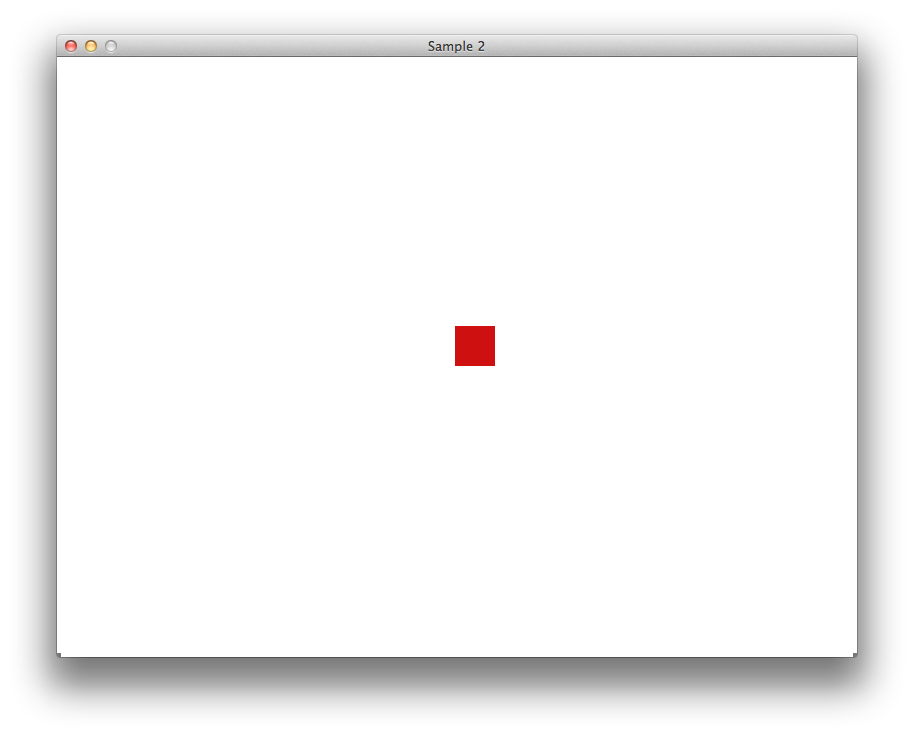
\includegraphics[width=0.8\textwidth]{./topics/control-flow/exercises/ClickGame.png} 
     \caption{The game in play}
     \label{fig:click_game}
  \end{figure}
  
  
  \begin{figure}[p]
    \csection{\ccode{clst:click_game}{What does this C code do?}{topics/control-flow/exercises/play_game.c}}
  \end{figure}
  \begin{figure}[p]
    \passection{\pascode{plst:click_game}{What does this Pascal code do?}{topics/control-flow/exercises/PlayGame.pas}}
  \end{figure}
  \clearpage
  
  \item Read the C code in \lref{clst:grid}, or the Pascal code in \lref{plst:grid}, and then answer the following questions:
  \begin{enumerate}
    \item What would be better names for the \texttt{i} and \texttt{j} variables?
    \item How many rectangles are drawn to the screen when this procedure is called?
    \item What does this code draw to the screen when it is called?
    \item How would you need to change the code to ensure that the rectangles were always square?
  \end{enumerate}
  \begin{figure}[h]
    \csection{\ccode{clst:grid}{What does this C code do?}{topics/control-flow/exercises/grid.c}}
  \end{figure}
  \begin{figure}[p]
    \passection{\pascode{plst:grid}{What does this Pascal code do?}{topics/control-flow/exercises/Grid.pas}}
  \end{figure}
  \clearpage
  
\end{enumerate}

\clearpage

Apply what you have learnt to the following tasks:
\begin{enumerate}
  \item Write a small program that will print the message `Hello World' to the Terminal `1 MILLION TIMES'... mmmmwwwahahahah\footnote{Dr Evil, Austin Powers, 1997}.
  \item Revisit your Circle Dimensions program from \cref{cha:storing_and_using_data} and adjust its implementation to make use of looping statements. The new output should display the radius, circle area, diameter, and circumference of circles with radius from 1.0cm to 1.0m at 0.25cm increments.
  \item Take your Times Table program from \cref{cha:storing_and_using_data}, and change it so that you can print a variable number of times. For example, have it print the 5 times table from 1 x 5 to 10 x 5, the 73 times table from 1 x 73 to 73 * 73, and the 42 times table from 1 x 42 to 7 * 42.  
  \item Implement the Guess that Number program, and test that your implementation works successfully.
  \item Take the adjusted Face Shape program from \cref{cha:storing_and_using_data}, and re-implement it so that it draws a new randomly places face each time through the loop in \texttt{Main}. SwinGame include a \texttt{rnd} function that can be used to generate a random number between 0 and 1, you can then multiply this by the Screen Width or Screen Height to get a random position.
  \item Try implementing some of the code reading questions. See if you can combine a few of them together to create a small game.
  
  \item Write a function called \texttt{Read Integer} that will read a number from the user. If the user does not enter a number the function will output the message `Please enter a number.', and will repeatedly ask the user to enter a number until they do so. Write a small program that tests if your function works correctly.
  
  \begin{figure}[h]
    \csection{You can use \texttt{scanf(" \%d", \&result) != 1} to read in the value entered into a \texttt{result} variable, and to check if it was a number\footnote{The \texttt{scanf} function returns the number of values successfully read. See \nameref{sub:c_terminal_input}.}, and you can use \texttt{scanf("\%*[\textasciicircum \textbackslash n]");} to flush the input when you get something other than a number.}    
  \end{figure}
  
  \item Use your \texttt{Read Integer} function to read two values from the user, and then output the larger of the two values.
  
  \item Use your \texttt{Read Integer} function to read in a number, and then print out a custom message for different values. For example, the value \texttt{42} could have the message `The meaning of life...', the value \texttt{73} could have the message `The best number, according to Dr. Sheldon Cooper', etc. Have at least five custom messages, and a default message when the user does not enter one of the selected values.
  
  \item Update your \emph{custom message} program, and have it ask the user if they want to quit at the end, allowing them to print multiple message values.
\end{enumerate}
  
\clearpage

If you want to further your knowledge in this area you can try to answer the following questions. The answers to these questions will require you to think harder, and possibly look at other sources of information.

\begin{enumerate}
  \item Implement a Number Guesser program that will guess numbers between 1 and 100. See the program description in \tref{tbl:number_guesser}

  \begin{table}[htbp]
  \centering
  \begin{tabular}{l|p{10cm}}
    \hline
    \multicolumn{2}{c}{\textbf{Program Description}} \\
    \hline
    \textbf{Name} & \emph{Number Guesser} \\
    \\
    \textbf{Description} & This program will work to \emph{guess} a number that the player is thinking of between 1 and 100. This will prompt the user to think of a number, and it will then guess using the following algorithm. The first guess will be 50 (the point half way between 1 and 100). The user will then enter a character to tell the computer how that value relates to the target value: `E' for equal, `L' for your guess is less than the target, and `G' for your guess is greater than the target. \newline

    When the guess is equal, a success message is output. \newline

    When the guess is less than the target the computer will take another guess that is half way between the guess and the pervious upper value (e.g. 1-100 = 50, 50-100 = 75, 75-100 = 87, 25-50 = 37, etc). \newline

    When the guess is larger than the target the computer will take another guess that is half way between the guess and the pervious lower value (e.g. 1-100 = 50, 1-50 = 25, 1-25 = 12, 50-75 = 62, etc). \newline

    Once the number is guessed (or the computer determines the player is cheating...) the program asks if the user wants to play again, and the process is repeated or the program quits.\\
    \hline
  \end{tabular}
  \caption{Description of the Number Guesser program.}
  \label{tbl:number_guesser}
  \end{table}

  \item Create a SwinGame project called \emph{Key Test}. See the description in \tref{tbl:key_test}.
  \begin{table}[htbp]
  \centering
  \begin{tabular}{l|p{10cm}}
    \hline
    \multicolumn{2}{c}{\textbf{Program Description}} \\
    \hline
    \textbf{Name} & \emph{Key Test} \\
    \\
    \textbf{Description} & This SwinGame will draw a filled red rectangle in the center of the screen when the user holds down the \textbf{r} key.\\
    \hline
  \end{tabular}
  \caption{Description of the Key Test program.}
  \label{tbl:key_test}
  \end{table}

  \item Extend the \emph{Key Test} program to draw other shapes when different keys are held down. For example, draw a filled circle when the user holds down the \textbf{c} key.

  \csection{You can call \texttt{key\_down(VK\_R)} to test if the `r' key is held down, then only draw the rectangle \emph{if} this key is held down.}
  
  \clearpage
  \item Color can be represented as consisting of three components: hue, saturation, and brightness. The hue component represents the color, the saturation is how much of this color is added to the white point, and the white point is controlled by the brightness and moves from black through grey to white. An illustration of this is shown in \fref{fig:color_wheel}.

\begin{figure}[htbp]
   \centering
   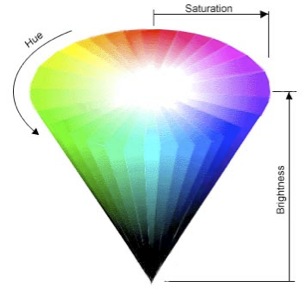
\includegraphics[width=0.3\textwidth]{./topics/control-flow/exercises/Color.png} 
   \caption{Color wheel showing HSB color}
   \label{fig:color_wheel}
\end{figure}

  SwinGame includes a \texttt{Draw Pixel} procedure that allows you to draw a single pixel on the screen. We can use this to draw a color banding across the screen by calculating the color for each pixel using SwinGame's \texttt{HSB Color} function.
  
  The structure of this program can be broken into three blocks: a \texttt{Color At} function, a \texttt{My Clear Screen} procedure and a \texttt{Main} procedure. This structure is shown in \fref{fig:my_clear_screen}.

  \begin{figure}[htbp]
     \centering
     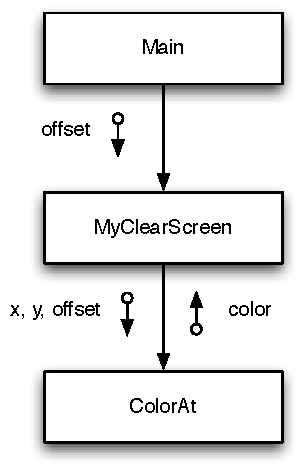
\includegraphics[width=0.3\textwidth]{./topics/control-flow/exercises/MyClearScreen.pdf} 
     \caption{Structure Chart for My Clear Screen}
     \label{fig:my_clear_screen}
  \end{figure}

\clearpage

The \texttt{Color At} function will be used to calculate the color for each pixel on the screen. This will be passed the \texttt{x} and \texttt{y} coordinates of the pixel (Integers) and an \texttt{offset}\footnote{Offset must have a value between 0 and 1 as the value for Hue must be between 0 and 1.} (a Double value). This function will call SwinGame's \texttt{HSB Color} function, passing in a hue calculated using the equation shown below, with saturation and brightness set to 0.9 and 0.8 respectively, and it will return the resulting color.

\begin{equation}
  hue = \frac{\displaystyle (Offset + \frac{x + y}{Screen Width + Screen Height})}{2}
\end{equation}

The equation will cycle the hue value between 0 and 1, covering the full spectrum of color. The \texttt{x + y} component will alter the color of the pixel based on its position on the screen, while the offset allows the program to change the color of the first pixel as time passes.

The \texttt{MyClearScreen} procedure will loop through all of the pixels across the screen (with x going from 0 up to (but not including) ScreenWidth()). This loop will select a single column of pixels on the screen, the pixels at the given x position. As this column has ScreenHeight() pixels you need an inner loop that loops from 0 to ScreenHeight(). Inside the inner loop the \texttt{x,y} values give you the coordinates of an individual pixel. You can now use the \texttt{Draw Pixel} procedure to draw this pixel, using the \texttt{Color At} function you wrote to determine its color.

Lastly the \texttt{Main} procedure will contain the standard game loop provided in the SwinGame project template. Replace the code within the loop so that it calls \texttt{My Clear Screen} then \texttt{Refresh Screen} and lastly \texttt{Process Events}. Within \texttt{Main} you need to maintain an offset value that you increment by a fixed value each loop\footnote{Trial this with different value < 1}, always ensuring the value is between 0 and 1. This offset is then passed to \texttt{My Clear Screen} when it is called.

See if you can use this information, and program design to create a small screensaver program. Experiment with different values and loops to see what effects you can create.
\end{enumerate}

